%!TEX program = xelatex
%!TEX root = ./thesis.tex

\subsection{Detailed environment specification}
We provide a detailed description of the experiment environments in this section. All of the environments are based on the "Ant" task~\cite{openaigym}. In the original "Ant" task, the agent receives a 111-dimensional state input and outputs a 8-dimensional action output. The agent's state consists of a 13-dimensional vector that represents its pose, a 14-dimensional vector that represents its velocity, and a 84-dimensional vector that represents related contack force. 

In the settings of the proposed environments, the agent receives not only the 111-dimensional state, but also a $64\times 64\times 1$ dimensional grayscale image observation. A sample image observation is shown in Figure~\ref{fig_ant_imgobs}.

\begin{figure}[H]
	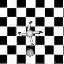
\includegraphics[width=0.5\textwidth]{images/ant_imgobs.png}
	\centering
	\caption{A sample image observation of the target environments}
\end{figure}\label{fig_ant_imgobs}

A basic task, namely "move0", is the same as the definition of "Ant" in OpenAI Gym~\cite{openaigym} except an extra image observation as state. The agent is required to move toward a specific direction $g_0=(1,0)$, and the reward at each time-step is given by:
\begin{align}
r = v_g + 1-c_p-c_c
\end{align}
Where $v_g=v \cdot g_0$ is the "forward reward", which rewards the agent for moving toward the goal direction.  $c_p$ is the control cost, which is the power that the agent is consuming, and $c_c$ is the contact cost, which penalizes the agent for strong collision. The episode terminates when the agent enters a unrecoverable state, such as  being turned over, or if the episode length reaches 1000 time-steps.

Other basic environments that might be used as source tasks are "move1", "move2", "move3", ..., "move7". This tasks are the same as "move0" except that the goal direction is different. The image observation is redundant for all these low-level tasks, because the agent only needs to move toward one specific direction.

The target tasks are design to be suitable for the definition of multi-modality and sparse-reward. We propose several multi-modality environments, including "moveg2", "moveg4", "moveg8", "movecont", "dynamicg4", "dynamiccont". These tasks requires the agent to learn not only from the state representation but also the image representation. We also propose sparse multi-modality environments: "reachg4" and "reachcont". The agent receives very sparse rewards in these environments compared with the previous environments, which have smooth reward function. The goal direction or location is represented by a sphere object in the image observation, thus the image observation plays a critical role in these tasks.
The set of all the proposed environments are described in table \ref{table_ant_envs}.


\begin{table}[!htbp]

\begin{center}
\begin{tabular}{|c|p{3cm}|p{4cm}|p{4cm}|}
\hline
Task name & Goal & Reward  &  Description \\
\hline\hline
move0 & velocity: $g_0=(1,0)$ &$ v_g+1-c_p-c_c$  & move toward a target direction \\
\hline
move1 & velocity: $g_1=(-1,0)$ &$ v_g+1-c_p-c_c$  & move toward a target direction\\
\hline
move2 & velocity: $g_2=(0,1)$ &$ v_g+1-c_p-c_c$  & move toward a target direction \\
\hline
move3 & velocity: $g_3=(0,-1)$ &$ v_g+1-c_p-c_c$  & move toward a target direction \\ 
\hline 
move4 & velocity: $g_4=(\sqrt{2}/2,\sqrt{2}/2)$ &$ v_g+1-c_p-c_c$  & move toward a target direction \\ 
\hline 
move5 & velocity: $g_5=(-\sqrt{2}/2,-\sqrt{2}/2)$ &$ v_g+1-c_p-c_c$  & move toward a target direction \\ 
\hline 
move6 & velocity: $g_6=(\sqrt{2}/2,-\sqrt{2}/2)$ &$ v_g+1-c_p-c_c$  & move toward a target direction \\ 
\hline 
move7 & velocity: $g_7=(-\sqrt{2}/2,\sqrt{2}/2)$ &$ v_g+1-c_p-c_c$  & move toward a target direction \\ 
\hline 
moveg2 & velocity samples from: $\{g_0,g_1\}$ &$ v_g+1-c_p-c_c$  & each episode has a random sampled goal direction \\ \hline
moveg4 & velocity samples from: $\{g_0,g_1,g_2,g_3\}$ &$ v_g+1-c_p-c_c$  & each episode has a random sampled goal direction \\ \hline
moveg8 & velocity samples from: $\{g_0,g_1, \dots,g_7\}$ &$ v_g+1-c_p-c_c$  & each episode has a random sampled goal direction \\ \hline
movecont & velocity samples from a continuous range of all unit directions&$ v_g+1-c_p-c_c$  & each episode has a random sampled goal direction \\ \hline
dynamicg8 &  velocity samples from: $\{g_0,g_1, \dots,g_7\}$ &$ v_g-c_p-c_c$  & the goal direction is re-sampled with probability 0.005 at each time-step  \\ \hline
dynamiccont & velocity samples from a continuous range of all unit directions &$ v_g-c_p-c_c$  & the goal direction is re-sampled with probability 0.005 at each time-step  \\ \hline
reachg4 & position samples from $\{g_0,g_1,g_2,g_3\}$ & $I(\lVert x-g\rVert_2^2<0.5) - 0.01$  & The agent is only rewarded when reaching a goal position\\ \hline
reachcont & position samples from the unit circle & $I(\lVert x-g\rVert_2^2<0.5) - 0.01$  & The agent is only rewarded when reaching a goal position\\ \hline

\end{tabular}
\end{center}
 \caption{Summary of Ant-based environments}
\end{table}\label{table_ant_envs}
